% Copyright (C) 2007 Technical University of Liberec.  All rights reserved.
%
% Please make a following refer to Flow123d on your project site if you use the program for any purpose,
% especially for academic research:
% Flow123d, Research Centre: Advanced Remedial Technologies, Technical University of Liberec, Czech Republic
%
% This program is free software; you can redistribute it and/or modify it under the terms
% of the GNU General Public License version 3 as published by the Free Software Foundation.
%
% This program is distributed in the hope that it will be useful, but WITHOUT ANY WARRANTY;
% without even the implied warranty of MERCHANTABILITY or FITNESS FOR A PARTICULAR PURPOSE.
% See the GNU General Public License for more details.
%
% You should have received a copy of the GNU General Public License along with this program; if not,
% write to the Free Software Foundation, Inc., 59 Temple Place - Suite 330, Boston, MA 021110-1307, USA.

% \chapter{Units}
% \begin{table}
%   \label{tab:units}
%   \begin{center}
%     \begin{tabular}{|l|c|}
%       \hline
%       \textbf{Quantity} & \textbf{Unit} \\
%       \hline 
%       lenght & $L$ \\
%       time & $T$ \\
%       conductivity & $ $ \\
%       concentration & $ $ \\
%       diffusivity & $ $ \\
%       \hline
%     \end{tabular}
%   \caption{The table of units used in the document.}
%   \end{center}
% \end{table}


%=====================================================
%                   TEST  1
%=====================================================

\section{Test 01 -- Steady flow}
\label{sec:test01}
This test considers steady Darcy flow in a cube domain which is cutted by 2D fractures which are further 
separated by a~1D channel in their cross section. The multidimensional connections between 1D, 2D and 3D 
elements are involved in the computation. A~Dirichlet boundary condition is prescribed for flow.
  \begin{itemize} 
    \item \emph{problem type} -- sequential coupling
    \item \emph{primary equation} -- steady mixed hybrid
  \end{itemize}

\subsection*{Geometry and boundary conditions}
A~cube with its side 1.0~\unitss{}{1}{} is cutted by two diagonal 2D fractures which are further separated 
by a~1D channel in their cross section.

Geometry parameters are defined for different physical domains. Thickness of the 2D fractures is set to 
1.0~\unitss{}{1}{} and the area of the cross section is set to 1.0~\unitss{}{2}{}. These parameters are 
unrealistic (the side of the cube is 1.0~\unitss{}{1}{} long) but it is compensated in the equation in 
the fraction with conductivity.

There are only simple Dirichlet boundary conditions. Pressure gradient in direction from one corner of the 
cube to the opposite corner is applied on all boundary faces of all dimensions.
%
\begin{figure}[htb!]
\centering
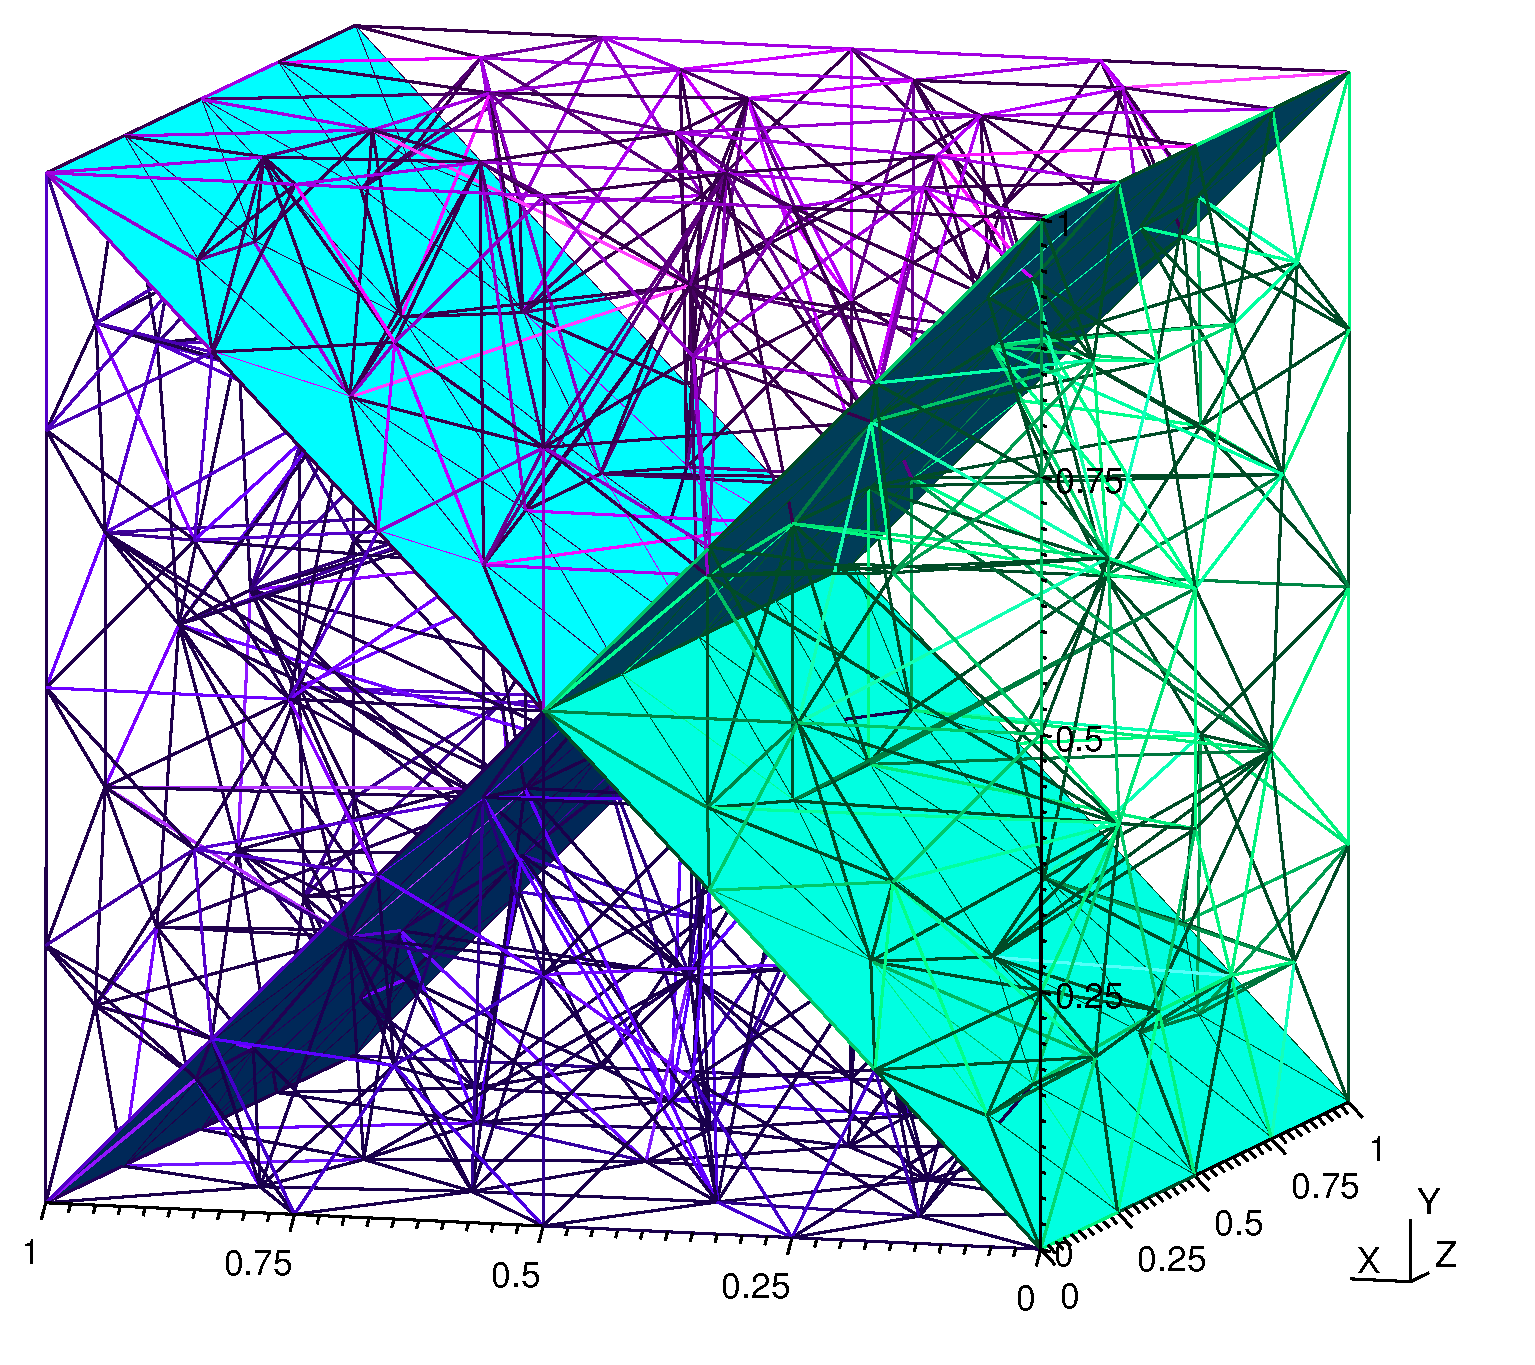
\includegraphics[width=13cm]{tests_graphics/01_mesh.pdf}
\caption{Test 01 -- mesh}
\label{fig:test1_mesh}
\end{figure}
%
%
\subsection*{Parameters}
\begin{itemize}
  \item \textbf{Cross section area:} 1D channel is set to 1.0~\unitss{}{2}{}.
  \item \textbf{Thickness:} 2D fractures are set to 1.0~\unitss{}{1}{}.
  \item \textbf{Conductivity:} The conductivity of materials:
    \begin{itemize}
      \item 1D channel is set to $K=10$~\unitss{}{1}{-1}.
      \item 2D fractures are set to $\mathbf{K}=\left(\begin{array}{cc} 1 & 0 \\ 0 & 1\end{array} \right)$~\unitss{}{1}{-1}.
      \item cube material is set to $\mathbf{K}=\left(\begin{array}{ccc} 0.1 & 0 & 0 \\ 0 & 0.1 & 0 \\ 0 & 0 & 0.1\end{array} \right)$~\unitss{}{1}{-1}.
    \end{itemize}
  \item There is no transport so there are not any other parameters.
\end{itemize}

\subsection*{Verification}
This test verifies solving steady Darcy flow by the mixed hybrid method. There are different dimensional connections 
which are 2D-3D connection between the cube and the flat fractures and 1D-2D connection between the 1D channel 
and the two flat fractures in their crossection. 

Following will not be commented in other examples and use of the functionalities will be considered apparent. No special test
programs are needed to test these as these are partially checked in the unit tests.

The input files \verb'flow_gmsh.con' and \verb'flow_vtk.con' give the same result, however the output is written in different 
formats. Also one can find an example of region set in \verb'flow_gmsh.con'.

Setting a Dirichlet boundary condition using piezometric head values is used in the input file \verb'flow_vtk_piezo.con'.
One can also notice using of the boundary set \verb'BOUNDARY' in this file. We use \emph{FieldFormula} to prescribe boundary
condition so this type of field and the function parser are also verified.

The remaining two files \verb'flow_old_vtk.con' and \verb'flow_vtk_fbc.con' use the obsolete way of defining boundary conditions.
The first one uses the old mesh without any named regions and the boundary condition file \verb'.fbc'. The second one combines
new mesh with named regions and the boudanry condition file created the old way. These tests ensure partially the backward 
compatibility of Flow123d with older input files.

%=====================================================
%                   TEST  2
%=====================================================

\section{Test 02 -- Steady flow in 2D and transport}
\label{sec:test02}
This test involves steady Darcy flow in 2D, connections of 1D-2D elements, Dirichlet boundary condition for flow and transport, 
transport of two substances with zero initial condition for concentration. There are actually two different cases computed in this test. 
Dual porosity and sorption features are present in the explicit transport. Dispersion is defined in the implicit transport.

The coefficient of diffusive transfer through a fracture (means between the fracture and the surrounding material) is set to 
zero so the substance cannot be diffused through the fracture's boundary.

  \begin{itemize} 
    \item \emph{problem type} -- sequential coupling 
    \item \emph{primary equation} -- steady mixed hybrid
    \item \emph{secondary equation} -- transport operator splitting (explicit), discontinuous Galerkin method (implicit)
  \end{itemize}

\subsection*{Geometry and boundary conditions}
The domain is two-dimensional slice through a part of a relief which involves several one-dimensional fractures.

Simple Dirichlet flow boundary condition is defined on left and right side where pressure heads are prescribed. 
There is no flow through the upper and lower boundary of the model. This all causes a flow along the x axis.

Dirichlet boundary condition for transport is prescribed on both sides as it is for flow boundary condition and 
the value of concentration is 1.0~\unitss{1}{-3}{} for both substances. Initial concentration of the substances 
is zero in the whole area. 
%
\begin{figure}[htb!]
\centering
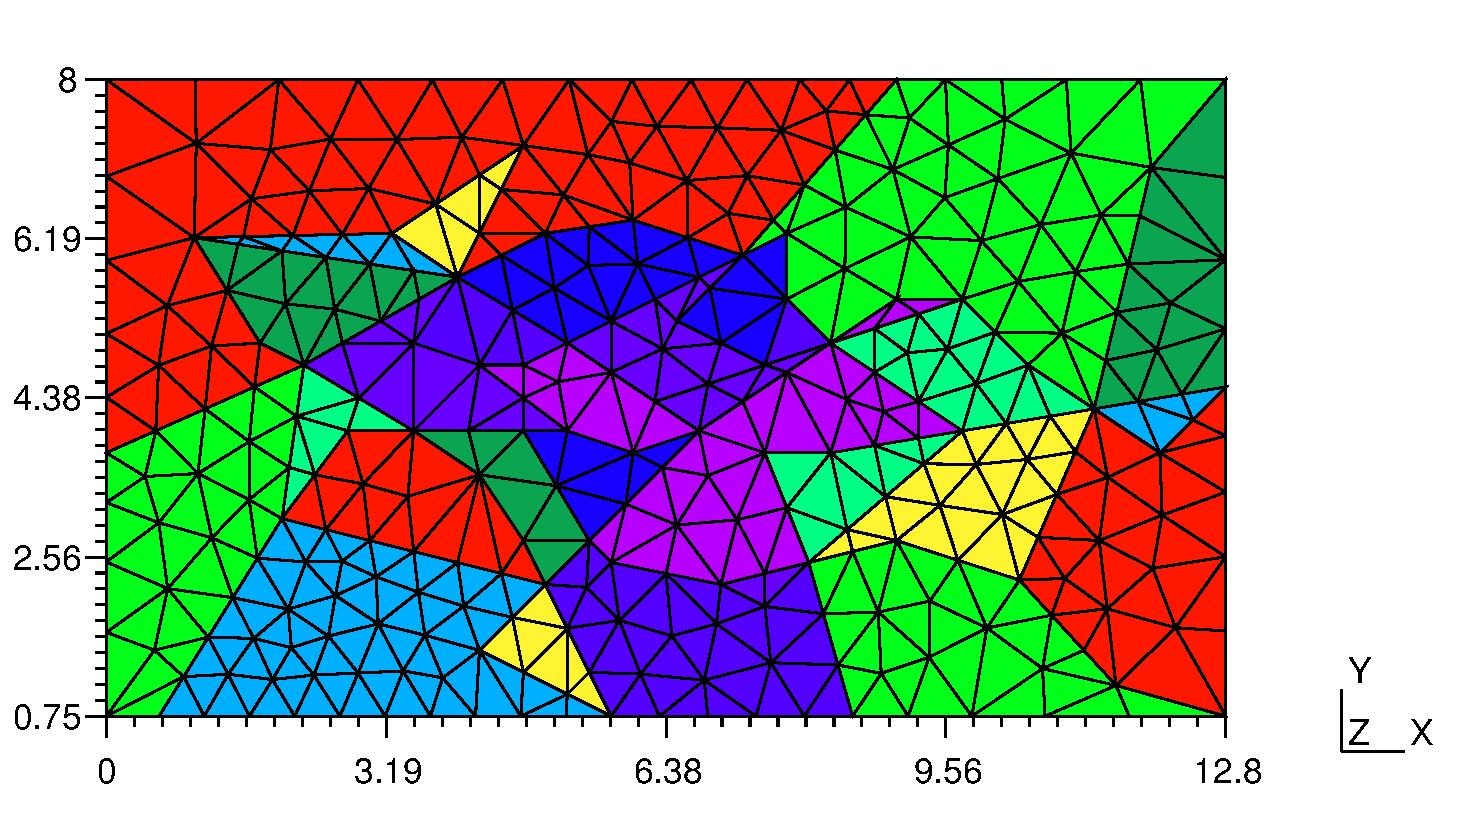
\includegraphics[width=15cm]{tests_graphics/02_mesh.pdf}
\caption{Test 02 -- mesh}
\label{fig:test2_mesh}
\end{figure}
%
%
\subsection*{Parameters}
The flow is steady and the transport is solved in time interval $(0,5.0)$~\unitss{}{}{1}. The output is written every 0.5~\unitss{}{}{1}. 
Time parameters for implicitly computed transport are the same only initial time step is set to 0.5~\unitss{}{}{1}.
\begin{itemize}
  \item \textbf{Cross section area:} 1D fractures are set to 1.0~\unitss{}{2}{}.
  \item \textbf{Thickness:} domain is set to 1.0~\unitss{}{1}{}.
  \item \textbf{Conductivity:} The conductivity of materials:
    \begin{itemize}
      \item fracture material is set to $K=10$~\unitss{}{1}{-1}.
      \item plane material is set to $\mathbf{K}=\left(\begin{array}{cc} 1 & 0 \\ 0 & 1\end{array} \right)$~\unitss{}{1}{-1}.
    \end{itemize}
  \item \textbf{Sorption:} The sorption parameters are for both materials equal:
    \begin{itemize}
      \item linear sorption isotherm parameter of the first substance is set to $k_l=0.02$.
      \item Freundlich sorption isotherm parameters of the second substance are set to $k_F=0.02$, $\alpha=0.5$  
    \end{itemize}
  \item \textbf{Dual porosity:} The dual porosity parameters are for both materials equal:
    \begin{itemize}
      \item mobile porosity coefficient is set to $0.25$
      \item immobile porosity coefficient is set to $0.25$
      \item nonequilibrium coefficient of both substances $0.01$
    \end{itemize}
  \item \textbf{Dispersion coefficients:} No dispersion is involved.
\end{itemize}

\subsection*{Verification}
This test verifies explicitly computed transport considering only convection with dual porosity and sorption and implicitly 
computed transport considering both convection and dispersion. Transport through 1D-2D element connections is computed in addition to the first test.



%=====================================================
%                   TEST  03
%=====================================================

\section{Test 03 -- Steady flow in 2D and transport}
\label{sec:test03}
This test differs from the previous one only by simpler structure of its geometry. It shows how the substace flows in the main fracture and divides in two other fractures. The substance spreads in the fractures much faster in comparision to transport in the plane.
\subsection*{Geometry and boundary conditions}
There is a plane with side 1.0 which is cutted by fractures. The main fracture divides in two other fractures.
\subsection*{Parameters}
The flow is steady and the transport is solved in time interval $(0,1.0)$. The output is written every 0.01. Initial time step for transport computed implicitly is set to 0.1 and the output is written every 0.1.

Other parameters are the same as in test 02.
\subsection*{Verification}
This test verifies the same features as the test 02 does but on a simpler geometry.



%=====================================================
%                   TEST  05
%=====================================================

\section{Test 05 -- Darcy flow boundary conditions}
\label{sec:test05}
There are three types of boundary conditions -- Dirichlet, Neumann and Robin that are tested. All three test have the same geometry and boundary conditions are derived from the same analytical solution.

We will prescribe analytical solution $u=xy$ of Laplace equation $-\Lapl{}u = 0$.
\begin{itemize} 
    \item \emph{problem type} -- sequential coupling 
    \item \emph{primary equation} -- steady mixed hybrid
  \end{itemize}

\subsection*{Geometry and boundary conditions}
The geometry is simple -- square plane in xy coordinates with corner points [0,0] and [1,1]. Each side has its own boundary regions called \verb0.bc_south0, \verb0.bc_east0, \verb0.bc_north0, \verb0.bc_west0.

\textbf{Dirichlet test.} All sides have pressure prescribed. These are south: $u_D=0$; east: $u_D=y$; north: $u_D=x$; west: $u_D=0$.

\textbf{Neumann test.} Two sides have pressure prescribed for the Dirichlet boundary condition: east: $u_D=y$; west: $u_D=0$. Two other sides have flux prescribed: south: $q_N=x$; north $q_N=-x$.

\textbf{Robin test.} Two sides have pressure prescribed  for the Dirichlet boundary condition: east: $u_D=y$; west: $u_D=0$.
For Robin boundary condition we get from the equation boundary pressure
\begin{equation} 
u_R=\frac{1+\sigma_R}{\sigma_R}x. 
\end{equation}
We choose $\sigma_R=0.5$ and then we get $u_R=-2x$ on the south side and $u_R=3x$ on the north side. 

\subsection*{Parameters}
\begin{itemize}
  \item \textbf{Conductivity:} on region \verb0plane0 is $1.0$~\unitss{}{1}{-1}.
  \item \textbf{Thickness:} on region \verb0plane0 is by default 1.0~\unitss{}{1}{}.
  \item There are no other regions, no transport so there are not any other parameters.
\end{itemize}

\subsection*{Verification}
This test verifies prescribing different types of boundary conditions.


%=====================================================
%                   TEST  06
%=====================================================

\section{Test 06 -- Coupling between dimensions in Darcy flow}
\label{sec:test06}
There are two tests -- \verb'flow_32d.con' for compatible coupling between 3D-2D and \verb'flow_21d.con' for compatible coupling between 2D-1D.

\begin{itemize} 
    \item \emph{problem type} -- sequential coupling 
    \item \emph{primary equation} -- steady mixed hybrid
  \end{itemize}

We will discuss both the geometry and parameters at once.

%
\begin{figure}[h!]
\centering
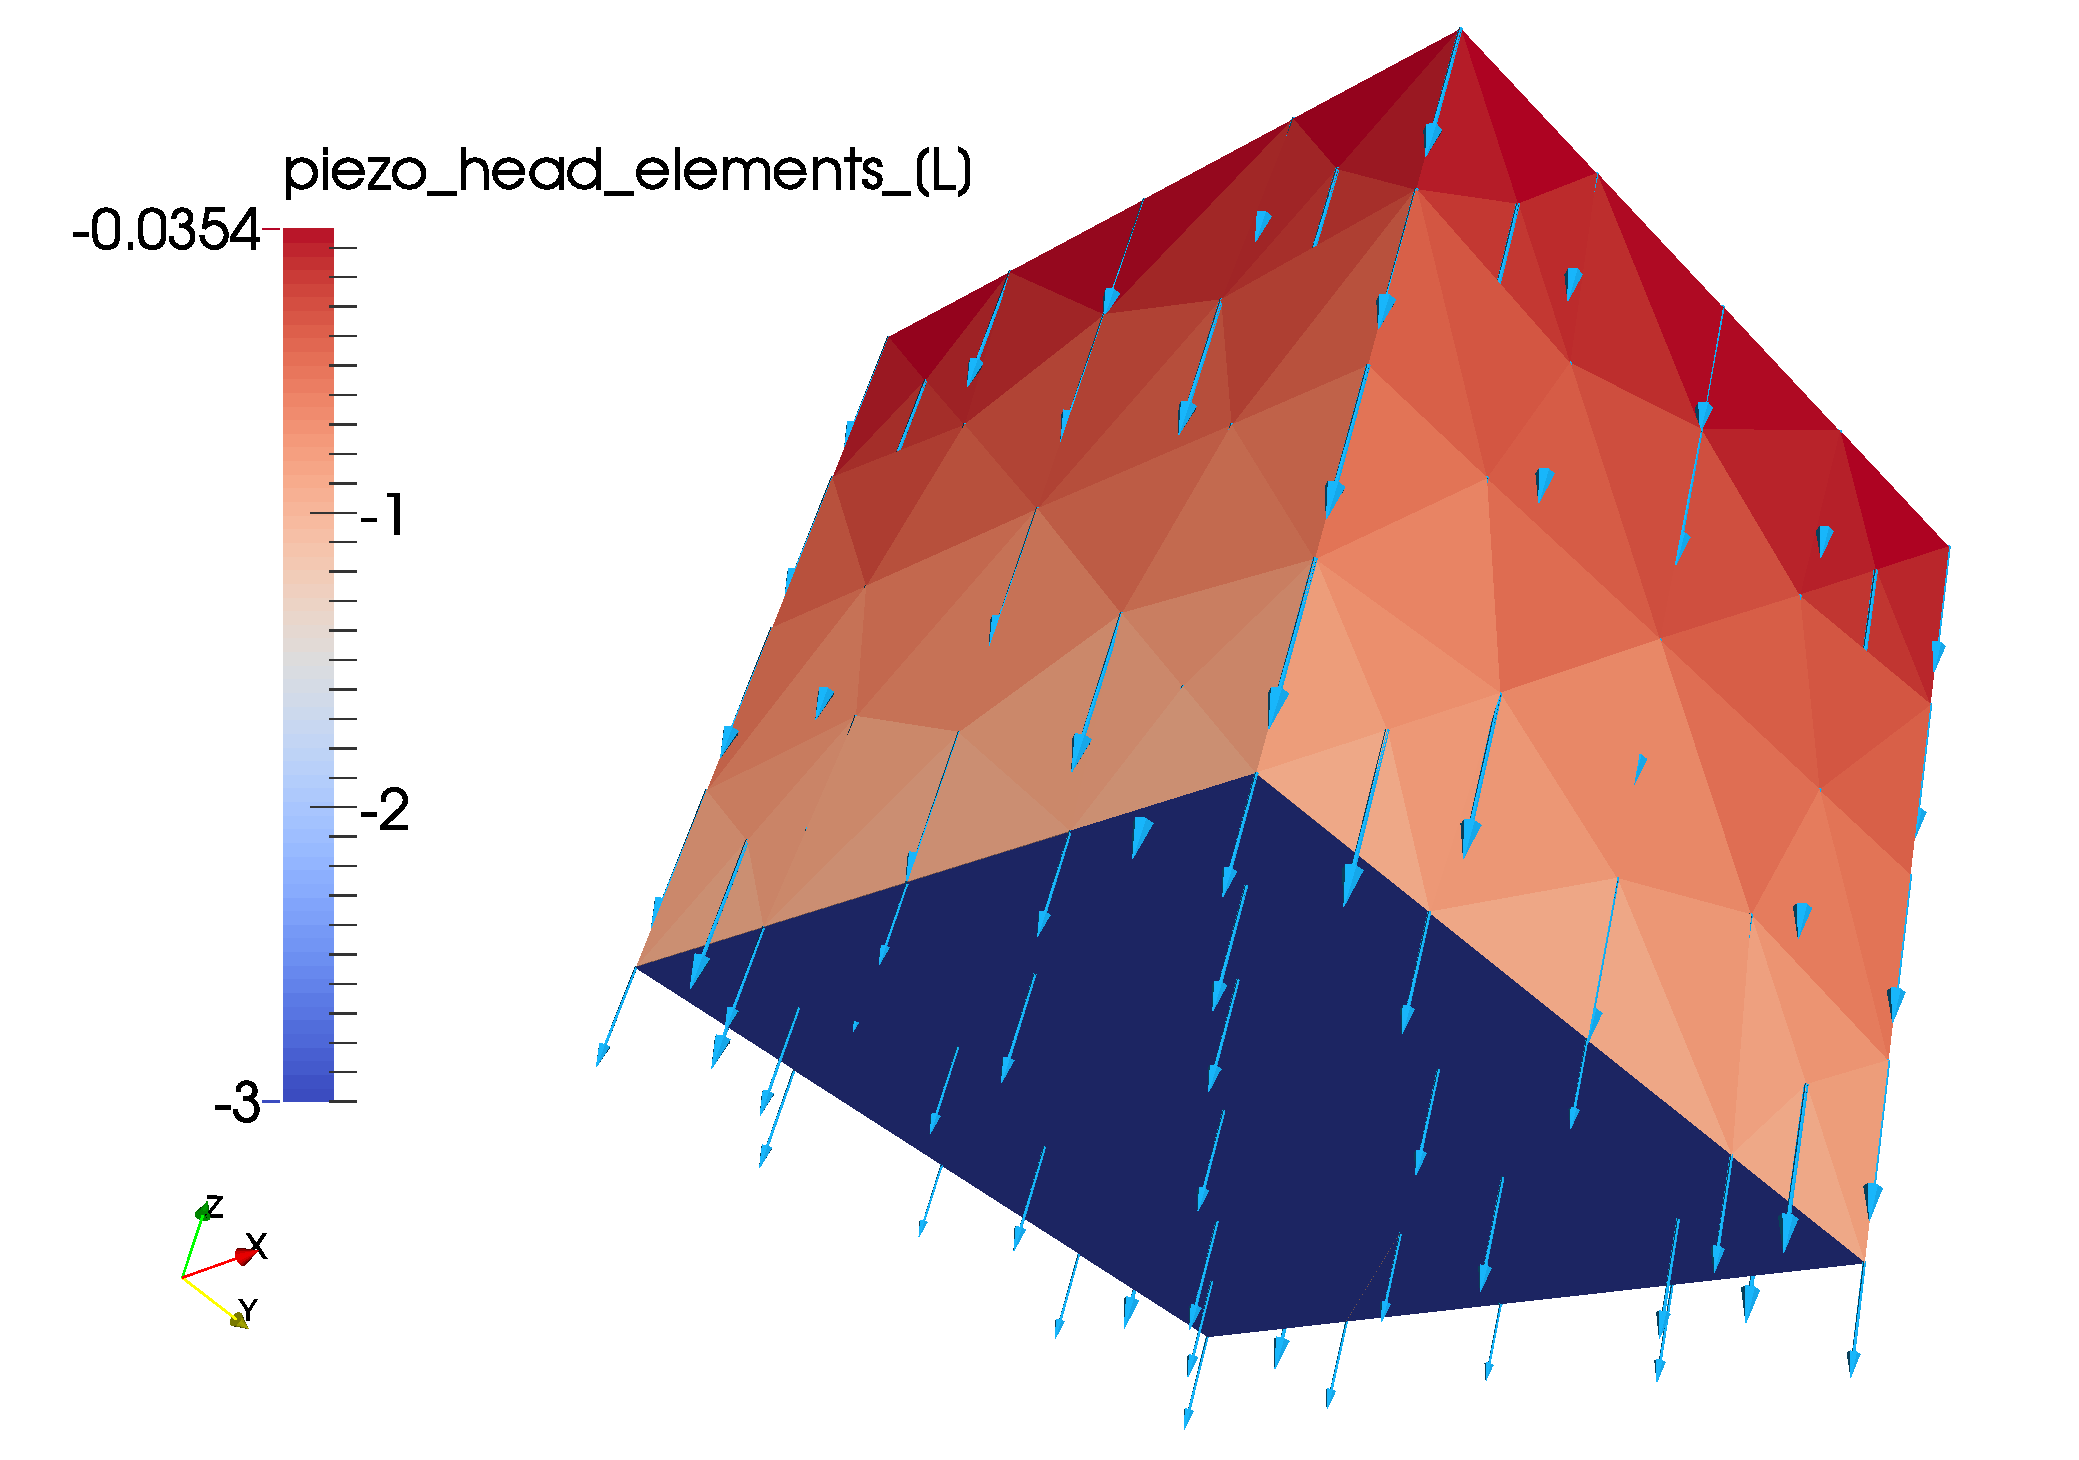
\includegraphics[width=0.6\textwidth]{tests_graphics/06_result_32d.pdf}
\caption{Test 06 -- solution. For verification see the blue plate where the constant 
         piezometric head -3~\unitss{}{1}{} is.}
\label{fig:test6_solution_32d}
\end{figure}
%
\textbf{3D-2D.}
There is a cube with vertices [0,0,0] [-1,-1,-1] which couples with a 2D crack in the bottom (i.e. $z=-1$~\unitss{}{1}{}).
We consider solution of the piezometric head in the cube $p_3(x,y,z) = z$. We will use it to 
prescribe Dirichlet boundary condition on the non-coupling parts of the cube.
There are no sources of a flow in the cube. 
We can write the outflow through the bottom of the cube in following term 
$q_{32} = \mathbf{q_3} \cdot \mathbf{n} = (- K_3 \nabla p_3(x,y,-1))\cdot \mathbf{n}$,
where $\mathbf{n}=(0,0,-1)$.
To obtain Laplace equation with zero right hand side on the 2D crack, we prescribe a new source 
term (\ref{eqn:test06_f2}) that eliminates the inflow coming from the cube.         
\begin{eqnarray}
    F_2 &=& \delta_2  f_2 + q_{32} = 0   \nonumber\\
    f_2(x,y) &=& -\frac{q_{32}}{\delta_2}   \label{eqn:test06_f2}.
\end{eqnarray}
When $\delta_2 = 10$~\unitss{}{1}{}, $K_3 = 2$~\unitss{}{1}{-1} are choosed then the source term is equal $f_2 = -0.2$~\unitss{}{}{-1}.
Homogenous Neumann condition is prescribed on the boundary of the fraction (zero outflow and inflow).

From the flow coupling equation we can get the piezometric head (\ref{eqn:test06_p2}) on the crack which we can verify.
\begin{eqnarray} 
     \sigma_{32}  ( p_3(x,y,-1) - p_2(x,y) ) &=& q_{32} \nonumber\\
     p_2(x,y) &=& -\frac{q_{32}}{\sigma_{32}} + p_3(x,y,-1) \label{eqn:test06_p2}.
\end{eqnarray}   
When $\sigma_{32} = 1$~\unitss{}{}{-1} is set then the piezometric head in the crack is constant and equal $p_2(x,y) = -3$~\unitss{}{1}{}
as we can see in figure \ref{fig:test6_solution_32d}.

%
\begin{figure}[h!]
\centering
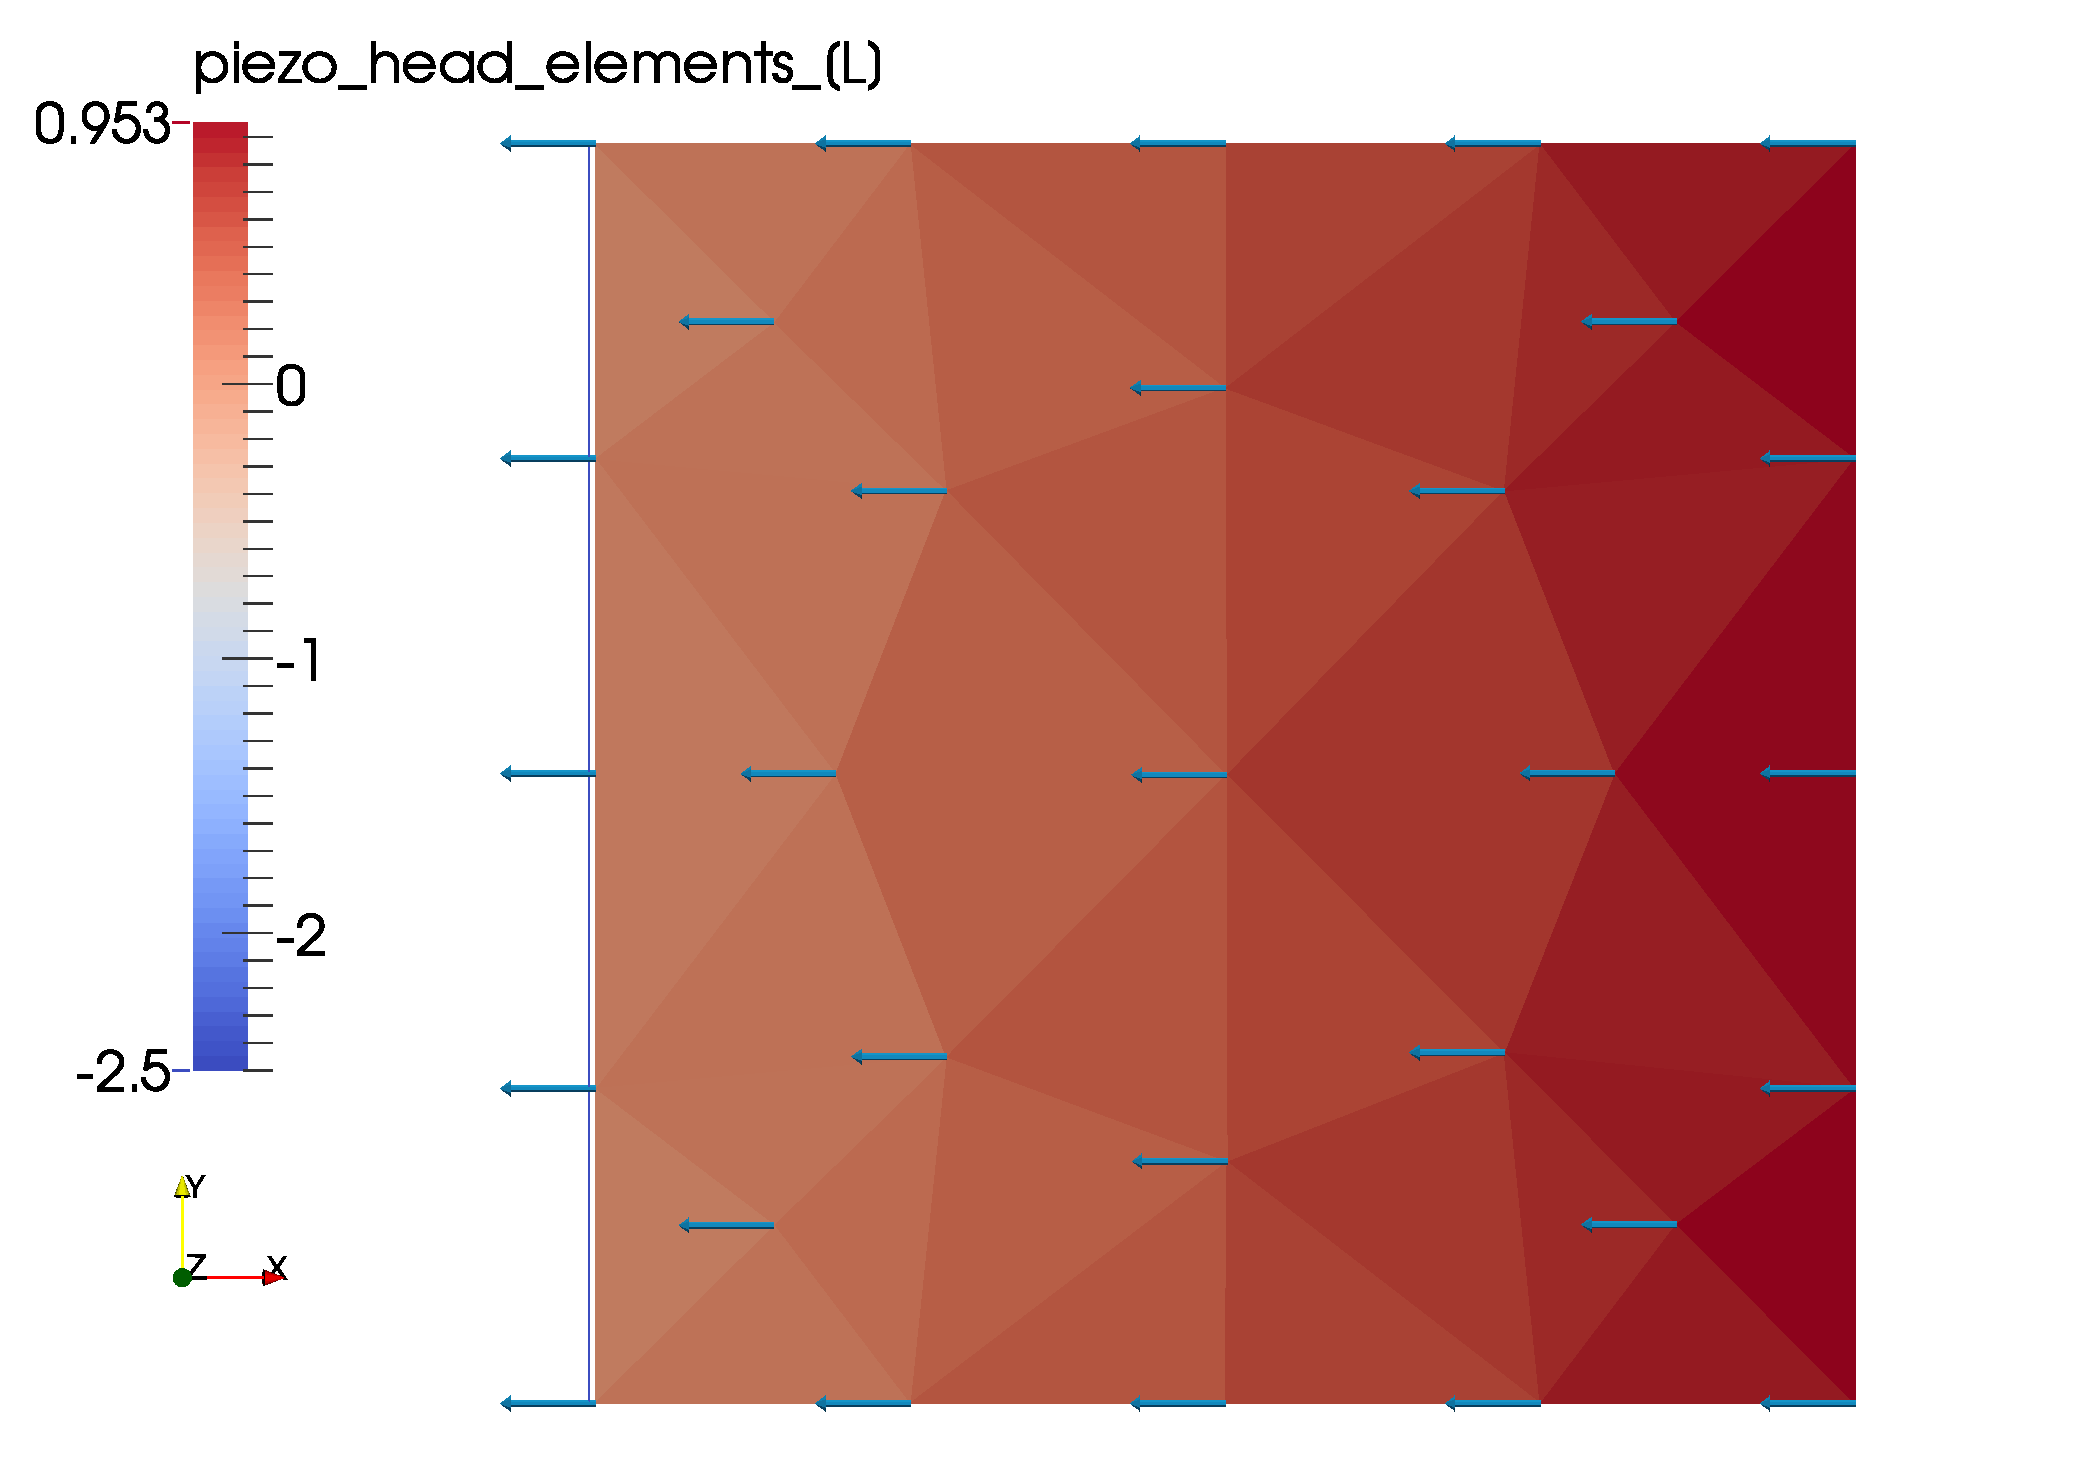
\includegraphics[width=0.6\textwidth]{tests_graphics/06_result_21d.pdf}
\caption{Test 06 -- solution. For verification see the blue channel on the left side of the plane 
         where the constant piezometric head -2.5~\unitss{}{1}{} is.}
\label{fig:test6_solution_21d}
\end{figure}
%
\textbf{2D-1D.}
The other tests geometry consists of a 2D crack in $xy$ plane with vertices [0,0] [1,1] and a 1D channel coupling with the crack on the left side ($x=0$). 
Everything is then analogical to the first test.
We consider solution of the pressure in the crack $p_2(x,y) = x$. We will use it to prescribe Dirichlet boundary condition on the non-coupling parts of the crack.
There are no sources of a flow in the crack. 
We can write the outflow through the left side of the crack in the following term $q_{21} = \mathbf{q_2} \cdot \mathbf{n} = (- \delta_2 K_2 \nabla p_2(0,y))\cdot \mathbf{n}$,
where $\mathbf{n}=(-1,0)$.
To obtain Laplace equation with zero right hand side on the channel, we prescribe a new source term (\ref{eqn:test06_f1}) that eliminates the inflow coming from the crack.         
\begin{eqnarray}
    F_1 &=& \delta_1  f_1 + q_{21} = 0   \nonumber\\
    f_1(x,y) &=& -\frac{q_{21}}{\delta_1}   \label{eqn:test06_f1}.
\end{eqnarray}
When $\delta_1 = 20$~\unitss{}{2}{}, $\delta_2 = 10$~\unitss{}{1}{} and $K_2 = 5$~\unitss{}{1}{-1} are choosed then the source term is equal $f_2 = -2.5$~\unitss{}{}{-1}.
Homogenous Neumann condition is prescribed on the boundary of the fraction (zero outflow and inflow).

From the flow coupling equation we can get the pressure (\ref{eqn:test06_p1}) on the plane which we can verify.
\begin{eqnarray} 
     \delta_2 \sigma_{21} ( p_2(0,y) - p_2(y) ) &=& q_{21} \nonumber\\
     p_1(y) &=& -\frac{q_{21}}{\delta_2 \sigma_{21}} + p_2(0,y) \label{eqn:test06_p1}.
\end{eqnarray}   
When $\sigma_{21} = 1$~\unitss{}{}{-1} is set then the pressure in the crack is constant and equal $p_1(y) = -2.5$~\unitss{}{1}{}
as we can see in the figure \ref{fig:test6_solution_21d}.

% \subsection*{Parameters}
% Parameters where discussed above.

\subsection*{Verification}
This test verifies correct communication between dimensions 3D-2D and 2D-1D in compatible coupling.
We can also observe the results in the \verb'water_balance' file. We should see that all the inflow 
to the cube should be fully compensated by the negative source. Homogenous Neumann boundary condition 
is prescribed on the crack so there should be no outflow or inflow through the boundary of the crack.
The situation in the second test is similar. The inflow to the crack should be fully compensated by 
the negative source in the channel which should have no other inflow or outflow.


%=====================================================
%                   TEST  8
%=====================================================

\section{Test 08 -- Steady Darcy flow with source}
\label{sec:test08}
This test is aimed at verifying steady Darcy flow with source which is prescribed by function formula. 
We will solve Laplace equation $-\Lapl{}u = f$ where source $f$ is prescribed by function $f = 2(1-y^2) + 2(1-x^2)$.
We can easily prove that (\ref{eqn:test8}) is the analytic solution by replacing it in the Laplace equation.
\begin{equation}
u = (1-x^2)(1-y^2) \label{eqn:test8}
\end{equation}

  \begin{itemize} 
    \item \emph{problem type} -- sequential coupling 
    \item \emph{primary equation} -- steady mixed hybrid
  \end{itemize}

\subsection*{Geometry and boundary conditions}
The domain is a square with opposite vertices $[-1,-1]$ and $[1,1]$. Zero dirichlet boundary condition is prescribed 
on all boundaries -- along the circumference of the square.
 
\subsection*{Parameters}
\begin{itemize}
  \item \textbf{Conductivity:} The conductivity of plane material is $1.0$~\unitss{}{1}{-1}.
  \item There are no other materials, no transport so there are not any other parameters.
\end{itemize}
%
\begin{figure}[h!]
\centering
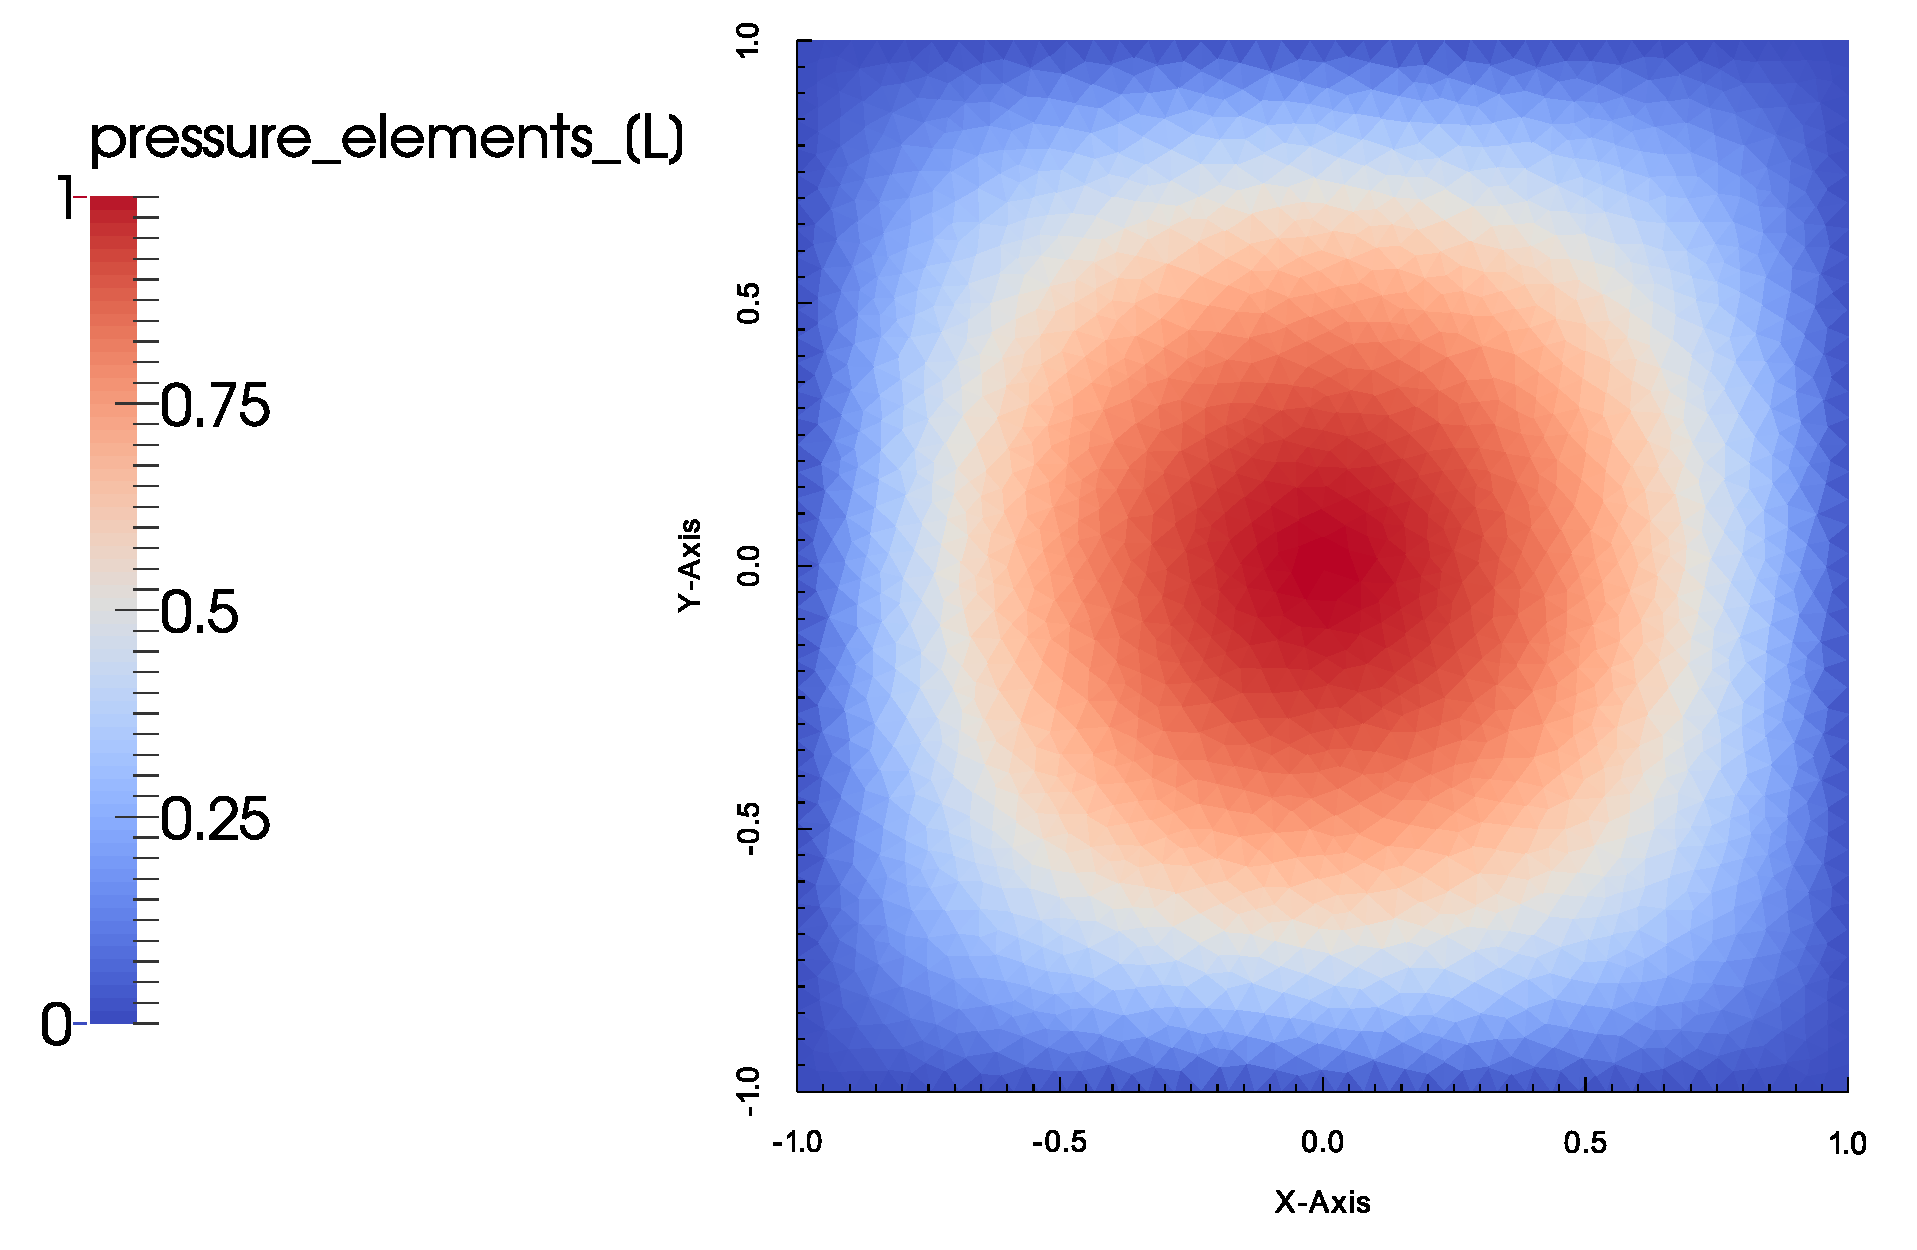
\includegraphics[width=0.8\textwidth]{tests_graphics/08_solution.pdf}
\caption{Test 08 -- solution. Distribution of the pressure matches the analytical solution (\ref{eqn:test8}).}
\label{fig:test8_solution}
\end{figure}
%
\subsection*{Verification}
The solution (pressure) is a paraboloid with a top in $[0,0,1]$ as we can see in the figure \ref{fig:test8_solution}. 
One can verify the equality in Paraview using the prepared state file.


%=====================================================
%                   TEST  10
%=====================================================

\section{Test 10 -- Unsteady flow in 2D}
\label{sec:test10}
Unsteady flow in 2D domain is simulated in this test and is computed by both mixed hybrid and 
lumped mixed hybrid method. No transport is involved. 

\begin{itemize} 
    \item \emph{problem type} -- sequential coupling
    \item \emph{primary equation} -- unsteady mixed hybrid, unsteady lumped mixed hybrid
  \end{itemize}

\subsection*{Geometry and boundary conditions}
The domain is a square with oposite vertices $[0,0]$ and $[1,1]$. Different Dirichlet boundary condition for 
pressure is prescribed on two opposite sides -- 0.0~\unitss{}{1}{} on the left and 100.0~\unitss{}{1}{} on the right.

\subsection*{Parameters}
The flow is solved in time interval $(0,0.5)$ with step 0.01~\unitss{}{}{1}. The output is written every 0.1~\unitss{}{}{1}.
\begin{itemize}
  \item \textbf{Conductivity:} The conductivity of plane material is $0.02$~\unitss{}{1}{-1}.
  \item Initial pressure is set to zero everywhere.
  \item There are no other materials, no transport so there are not any other parameters.
\end{itemize}

\subsection*{Verification}
This test verifies two different numerical methods -- the problem is computed by both mixed hybrid and lumped mixed hybrid method.

%=====================================================
%                   TEST  11
%=====================================================

\section{Test 11 -- Radioactive decay chain with more branches}
8 isotopes are members of considered decay chain with three branches. Transport boundary conditions does not matter 
because zero presure gradient is considered. Final concentrations of all isotopes except C decrease to zero after 20 
time steps, whereas C concentration grows to 0.36.
\[
 E\xrightarrow{}D\xrightarrow{}F\xrightarrow{}B
 \quad
 \begin{matrix}
    0.2B\xrightarrow{}A & A\xrightarrow{}G \\
    0.6B\xrightarrow{}H & H\xrightarrow{}G \\
    0.2B\xrightarrow{}G &\\
 \end{matrix}
 \quad
 G\xrightarrow{}C 
\]

\begin{itemize} 
    \item \emph{problem type} -- sequential coupling
    \item \emph{primary equation} -- steady mixed hybrid
    \item \emph{secondary equation} -- transport operator splitting
    \item \emph{reactions} -- linear reactions
  \end{itemize}

\subsection*{Geometry}
The domain is a prism which base is a right-angled triangle with its ordinates 3.0~\unitss{}{1}{}. 
There are only three tetrahedron elements in the mesh.

\subsection*{Parameters}
The flow is steady and the transport is solved in time interval $(0,10.0)$~\unitss{}{}{1}. The output is written every 0.5~\unitss{}{}{1}.

Half-lives are equal to 0.5 for all isotopes. Initial concentrations are summarized in the table below:
  \begin{center}
    \begin{tabular}[c]{|l|c|c|c|c|c|c|c|c|}
      \hline
      isotop & A & B  & C & D & E & F & G & H \\[4pt]
      initial concentration & 0.01 & 0.02 & 0.03 & 0.04 & 0.05 & 0.06 & 0.07 & 0.08 \\[4pt]
      \hline
    \end{tabular}
  \end{center}


\subsection*{Verification}


%=====================================================
%                   TEST  12
%=====================================================

\section{Test 12 -- Radioactive decay}
There are actually two tests of the radioactive decay. The first one considers first order reaction of two isotopes 
determined by kinetic constant and the other one describes radioactive decay chain of three isotopes.

\begin{itemize} 
    \item \emph{problem type} -- sequential coupling
    \item \emph{primary equation} -- steady mixed hybrid
    \item \emph{secondary equation} -- transport operator splitting
    \item \emph{reactions} -- linear reactions
  \end{itemize}

\subsection*{Geometry and boundary conditions}
The domain is a prism which base is a right-angled triangle with its ordinates 3.0 units long. There are then only three tetrahedron elements in the mesh.

There are two Dirichlet boundary conditions for flow prescribed.

\begin{itemize}
  \item \textbf{Conductivity:} The conductivity of the prism material is $0.01$~\unitss{}{1}{-1}. 
  \item There is no other parameter for flow or transport.
\end{itemize}



\subsection{First order reaction determined by kinetic constant}
The only linear reaction between D and F substances.
\[
D\xrightarrow{k}F
\]

\subsection*{Parameters}
The flow is steady and the transport is solved in time interval $(0,10.0)$. The output is written every 0.5~\unitss{}{}{1}.  
\begin{itemize}
  \item \textbf{Substances:} 6 substances to be transported -- A, B, C, D, E, F
  \item \textbf{Kinetic constant:} $k = 0.277258872$
\end{itemize}

\subsection*{Verification}

\subsection{Radioactive decay chain}
The considered radioctive decay chain is:
\[
 D\xrightarrow{t_{1/2,D}}F\xrightarrow{t_{1/2,F}}B
\]
\subsection*{Parameters}
Time parameters are the same as they are above.
\begin{itemize}
  \item \textbf{Substances:} 6 substances to be transported -- A, B, C, D, E, F
  \item \textbf{Decay half-lives:} $t_{1/2,D} = t_{1/2,F} = 2.5$
\end{itemize}

\subsection*{Verification}

% Both following tests are realized without combination with transport (zero pressure gradient).
% verification of:
% - first order reaction A->B determined by kinetic constant,
% -- 6 chemical species (A, B, .., F) are transported but just 2 of them take a part in considered first order kinetic reaction wich looks as follows
% --- D->F, appropriate kinetic constant is k = 0.277258872.
% --- Initail conditions look as follows, A(0) = 0.01, B(0) = 0.02, C(0) = 0.03, D(0) = 0.04, E(0) = 0.05, F(0) = 0.06.
% --- Transport boundary conditions does not matter because zero presure gradient is considered.
% --- Final concentrations of all isotopes except A, B, C, E do not change. Concentrations of D decreases to 0.003. Concentration of F increase to 0.85 in 20 time steps.

% - narrow radioctive decay chain without branches, A -> B -> C,
% -- 6 isotopes (A, B, .., F) are transported but just 3 of them are members of considered decay chain which looks as folows
% --- D->F->B
% --- Initail conditions look as follows, A(0) = 0.01, B(0) = 0.02, C(0) = 0.03, D(0) = 0.04, E(0) = 0.05, F(0) = 0.06.
% --- Transport boundary conditions does not matter because zero presure gradient is considered.
% --- Final concentrations of all isotopes except A, C, E do not change. Concentrations of D and B decrease to 0.004 and 0.012 respectively. Concentration of B increase to 0.1 in 20 time steps.

%=====================================================
%                   TEST  13
%=====================================================

\section{Test 13 -- Solute mixing on the edge}
This test realizes mixing of substances on the edges of planes and also does quantitative test on a trivial 
transport problem. The problem is computed with both explicit and implicit transport.

\begin{itemize} 
    \item \emph{problem type} -- sequential coupling 
    \item \emph{primary equation} -- steady mixed hybrid
    \item \emph{secondary equation} -- transport operator splitting (explicit), discontinuous Galerkin method (implicit)
  \end{itemize}

\subsection*{Geometry and boundary conditions}
The domain is a fork where the main branch with the incoming solute is 5~\unitss{}{1}{} long and lies in 
the $xy$ plane. Then it is divided into two other branches $5\sqrt{2}$~\unitss{}{1}{} long, one with 
positive and the another with negative $z$ coordinate. There are different conductivities in each branch.

Dirichlet boundary conditions for flow and transport are prescribed at the beginning of the main 
plane ($x=0$~\unitss{}{1}{}) and at the ends of the secondary branches ($x=10$~\unitss{}{1}{}).

flow: $h_D=-x-z+10.0$ which gives 10.0~\unitss{}{1}{} at point [0,0,0] and $\pm5$~\unitss{}{1}{} at points [10,0,$\mp5$]\\
transport: concentration is 1.0 at point [0,0,0] and 0.0 at points [10,0,$\mp5$]

Initial concentration of the substances is zero in the whole area. 
%
\subsection*{Parameters}
The flow is steady and the transport is solved in time interval $(0,100.0)$~\unitss{}{}{1}. 
The output is written every 5~\unitss{}{}{1}. 
Time parameters for implicitly computed transport are the same only initial time step and output time is set to 5.0~\unitss{}{}{1}.
\begin{itemize}
  \item \textbf{Thickness:} all planes are set to 1.0~\unitss{}{1}{}.
  \item \textbf{Conductivity:} The conductivity of materials (isotropic planes):
    \begin{itemize}
      \item main branch (material num. 17): $K=1$~\unitss{}{1}{-1}.
      \item branch (positive $z$, material num. 18): $K=0.1$~\unitss{}{1}{-1}.
      \item branch (negative $z$, material num. 19): $K=0.1$~\unitss{}{1}{-1}.
    \end{itemize}
  \item \textbf{Dispersion coefficients:} Default parameters are set in implicit transport, so no dispersion is present. 
        For more details see \hyperlink{IT::TransportDG-BulkData}{TransportDG\_BulkData} in the input reference.
\end{itemize}
%
\begin{figure}[!h]
    \centering
    \begin{subfigure}[b]{0.45\textwidth}
        \centering
        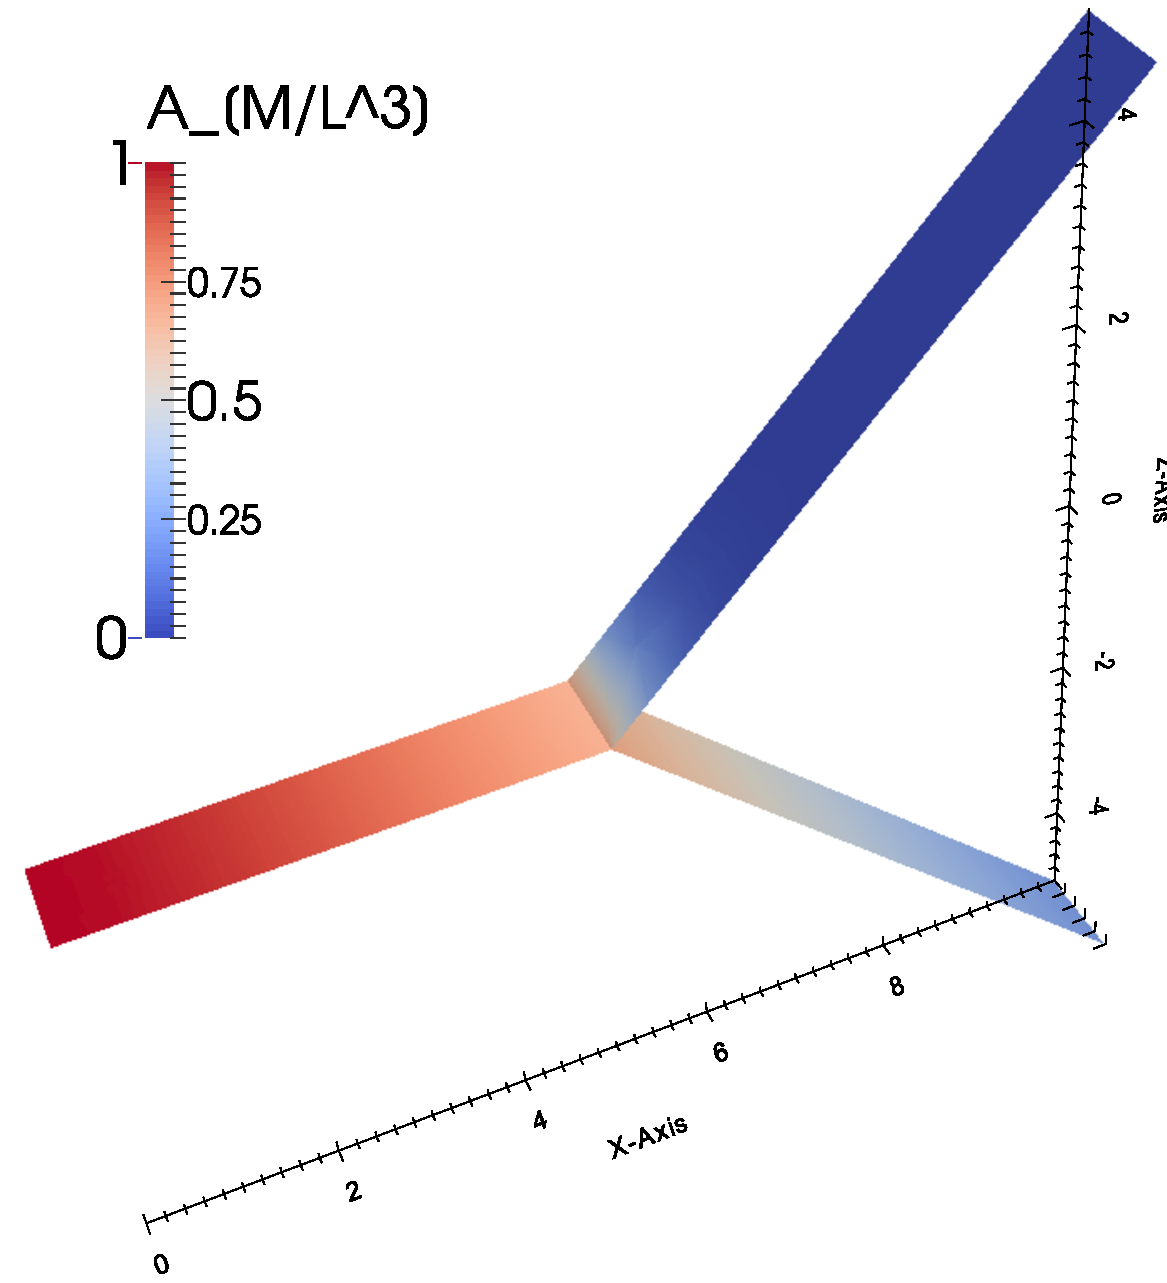
\includegraphics[width=\textwidth]{tests_graphics/13_solution_t2.pdf}
        \caption{Solution at time 10~\unitss{}{}{1}.}
        \label{fig:test13_a}
    \end{subfigure}
    ~
    \begin{subfigure}[b]{0.45\textwidth}
        \centering
        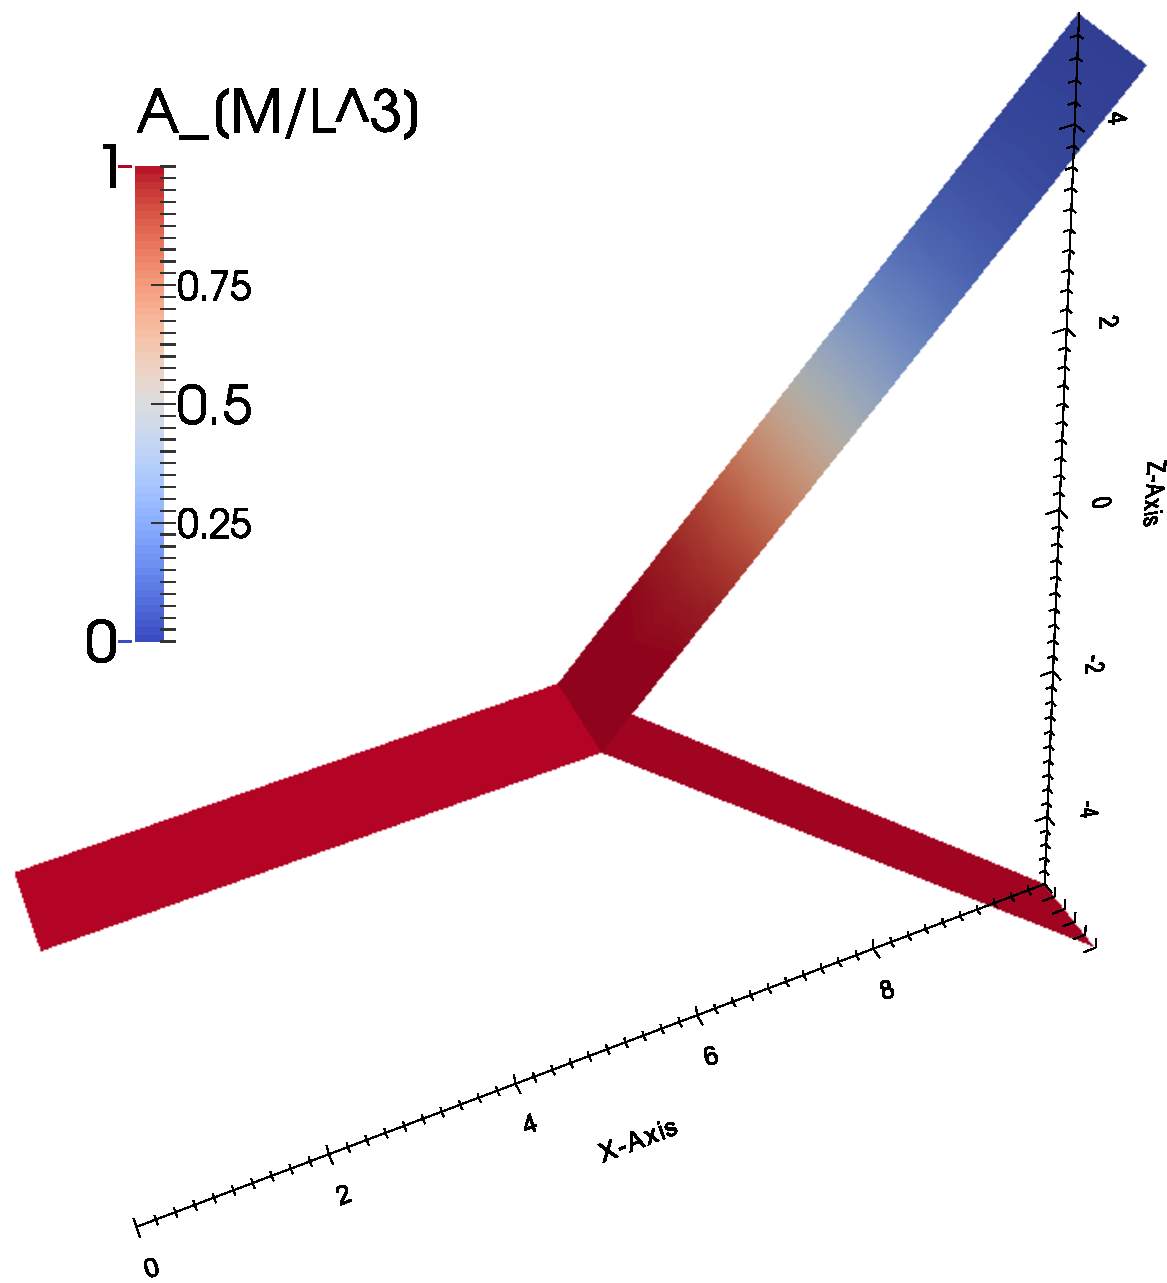
\includegraphics[width=\textwidth]{tests_graphics/13_solution_t10.pdf}
        \caption{Solution at time 10~\unitss{}{}{1}.}
        \label{fig:test13_b}
    \end{subfigure}
    \caption{Test 13 -- mesh}
  \label{fig:test13}
\end{figure}
%
\subsection*{Verification}
This test verifies qualitatively both the problem of flow and transport. We can see the influence of smaller conductivity 
in upper branch in the figure \ref{fig:test13}. The concentration of the substance spreads slower in the upper branch than 
in the lower one.

%=====================================================
%                   TEST  14
%=====================================================

\section{Test 14 -- Variable transport boundary condition}
We consider a time variable boundary condition for transport in this test. Steady flow with constant velocity is caused by a pressure 
gradient from one side of a 2D strip to the another. Dirichlet boundary condition for transport evolving in time is prescribed on the 
right side using set of older \verb'.tbc' files. 

\begin{itemize} 
    \item \emph{problem type} -- sequential coupling, 
    \item \emph{primary equation} -- steady mixed hybrid
    \item \emph{secondary equation} -- transport operator splitting (explicit), discontinuous Galerkin method (implicit)
  \end{itemize}

\subsection*{Geometry and boundary conditions}

Dirichlet boundary condition for pressure is prescribed $h_D = x$ all around the plane and causes constant flow from right to left 
(pressure prescribed on the upper and lower sides are equal along x axis so causes no flow). Transport boundary condition has 
the same prescribtion as for the pressure, only the values evolves in time.

Initial concentration is zero on the whole plane. Two pulses of nonzero concentration are applied on the boundary. The changes 
of the boundary condition at specified times are shown in the following table:
%
\begin{center}
  \begin{tabular}{|l|c|c|c|c|c|}
    \hline
    time \units{}{}{1} & $0$ & $1$ & $3$ & $6$ & $7$\\
    concentration & $0$ & $20$ & $0$ & $40$ & $0$\\
    \hline
  \end{tabular}
\end{center}

\begin{figure}[htb!]
\centering
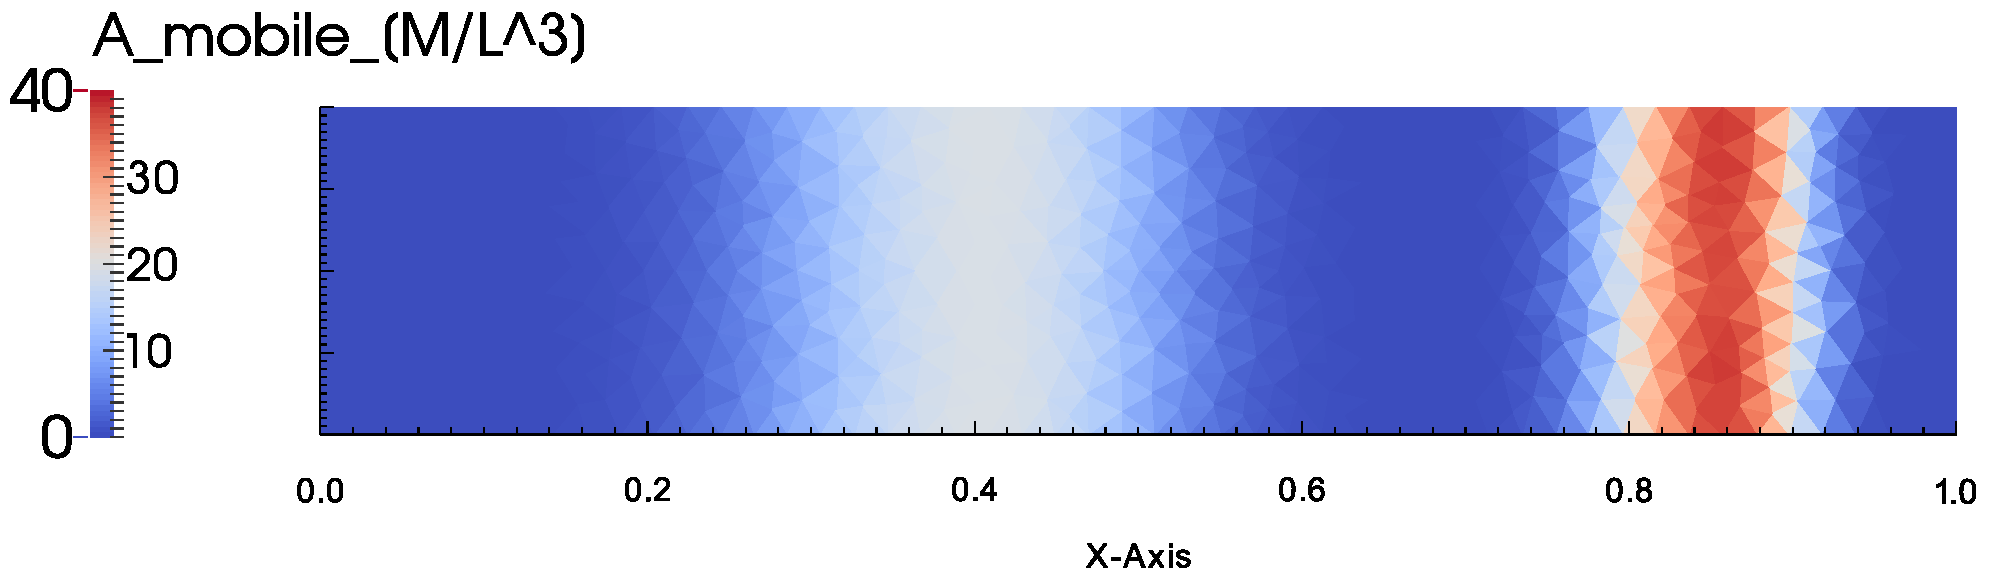
\includegraphics[width=15cm]{tests_graphics/14_solution.pdf}
\caption{Test 14 -- solution at time 8.0~\unitss{}{}{1}.}
\label{fig:test14_mesh}
\end{figure}
%
%
\subsection*{Parameters}
The flow is steady and the transport is solved in time interval $(0,10.0)$~\unitss{}{}{1}. The output is written every 
1.0~\unitss{}{}{1}. Time parameters for implicitly computed transport are the same only initial time step is set to 1.0~\unitss{}{}{1}.
%
\begin{itemize}
  \item \textbf{Thickness:} all planes are set to 1.0~\unitss{}{1}{}.
  \item \textbf{Conductivity:} The conductivity of material (isotropic plane): $K=0.1$~\unitss{}{1}{-1}.
  \item \textbf{Dispersion coefficients:} Default parameters are set in implicit transport, so no dispersion is present. 
        For more details see \hyperlink{IT::TransportDG-BulkData}{TransportDG\_BulkData} in the input reference.
\end{itemize}
%

\subsection*{Verification}
This test verifies that the transport boundary condition can evolve in time. We use old \verb'.tbc' for description 
of the transport boundary condition but all other possibilities work also.


%=====================================================
%                   TEST  15
%=====================================================

\section{Test 15 -- Unsteady flow with transport}
Transport of a single pulse of concentration moving along a 2D strip is solved. This test involves unsteady flow computed by lumped hybrid method, transport is solved both with explicit and implicit (involves dispersion) scheme.
 
\begin{itemize} 
    \item \emph{problem type} -- sequential coupling, 
    \item \emph{primary equation} -- unsteady lumped mixed hybrid
    \item \emph{secondary equation} -- transport operator splitting (explicit), discontinuous Galerkin method (implicit)
  \end{itemize}

\subsection*{Geometry and boundary conditions}
The domain is a 2D strip with dimensions $1.0$x$16.0$. Zero Dirichlet boundary for flow is prescribed at $x=0$, zero Neumann boundary is elsewhere. 

Dirichlet transport boundary condition is set on the left side to 10.0 only at the beginning. Then is this boundary condition zero.

\subsection*{Parameters}
Initial pressure is zero everywhere. 
The source is prescribed with function $f=-x$ along the strip.
%
\begin{itemize}
  \item \textbf{Thickness:} all planes are set to 1.0~$L$.
  \item \textbf{Conductivity:} The conductivity of material (isotropic plane): $K=1.0$.
  \item \textbf{Source formula:} $f = -x$
  \item \textbf{Diffusivity coefficients:} are used in implicit transport wth dispersion. 
	Default parameters are set ($d_m=1e-6$, others are zero, see manual or parameters in test02 in ~\ref{sec:test02}).
\end{itemize}
%
\begin{figure}[htb!]
\centering
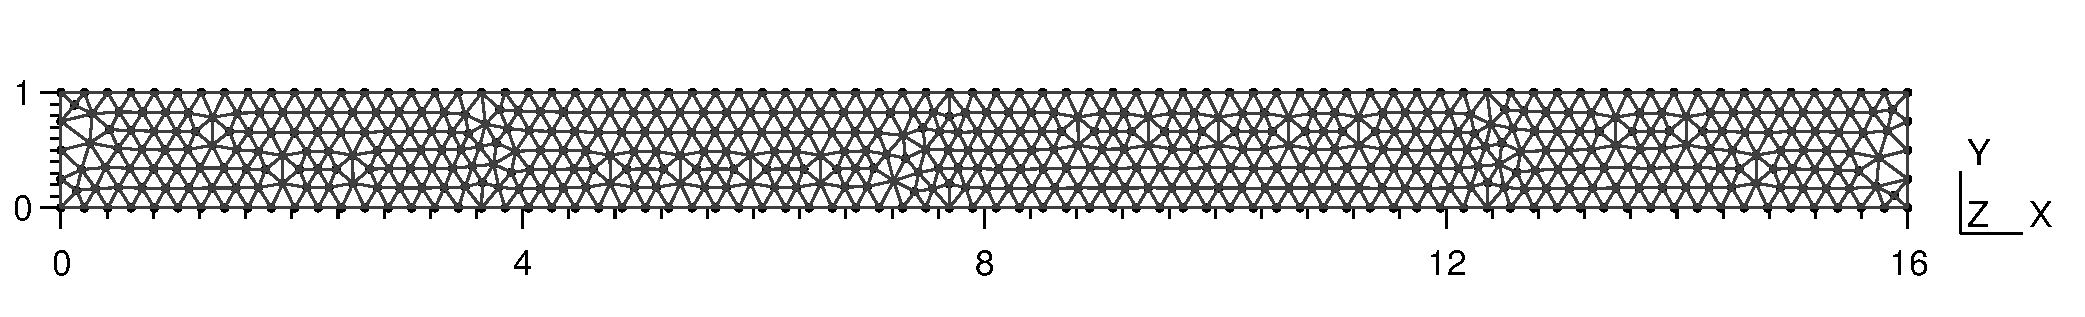
\includegraphics[width=15cm]{tests_graphics/15_mesh.pdf}
\caption{Test 15 -- mesh}
\label{fig:test15_mesh}
\end{figure}
%
%
\subsection*{Verification}
The test is similar to the test 10 but here in addition the computation of a transport in an unsteady flow field is verified.


%=====================================================
%                   TEST  16
%=====================================================

\section{Test 16 -- Substance concentration source in transport}
This test include a source of concentration of a substance. The domain is a 2D strip in vertical direction. There is a steady flow with constant velocity in the vertical direction. Two sources are situated on two elements at the top of the strip and the substance is transported down along the strip. The concentration values of the sources are defined in the \verb0tso0 input file.

\begin{itemize} 
    \item \emph{problem type} -- sequential coupling, 
    \item \emph{primary equation} -- steady mixed hybrid
    \item \emph{secondary equation} -- transport operator splitting
  \end{itemize}

\subsection*{Geometry}


\subsection*{Parameters}

\subsection*{Verification}



%=====================================================
%                   TEST  17
%=====================================================

\section{Test 17 -- Radioactive decay -- Pade approximation}
This test solves radioactive decay chain of five isotopes using Pade approximation.
The considered radioctive decay chain is:
\[
 A\xrightarrow{t_{1/2,A}}B\xrightarrow{t_{1/2,B}}C\xrightarrow{t_{1/2,C}}D\xrightarrow{t_{1/2,D}}E
\]

\begin{itemize} 
    \item \emph{problem type} -- sequential coupling, 
    \item \emph{primary equation} -- steady mixed hybrid
    \item \emph{secondary equation} -- transport operator splitting
    \item \emph{reactions} -- Pade approximation
  \end{itemize}

\subsection*{Geometry}
The geometry and material and transport parameters are the same as in test 12.


\subsection*{Parameters}
\begin{itemize}
  \item \textbf{Substances:} 5 substances to be transported -- A, B, C, D, E
  \item Polynomial degree of the nominator and the denominator of Pade approximation is~3.
  \item \textbf{Decay half-lives:} 
    \begin{tabular}[c]{|c|c|c|c|}
      \hline
      $t_{1/2,A}$ & $t_{1/2,B}$  & $t_{1/2,C}$ & $t_{1/2,D}$\\[4pt]
      $1.3863$ & $2.3105$ & $1.5403$ & $1.1552$\\[4pt]
      \hline
    \end{tabular}
\end{itemize}

\subsection*{Verification}


%=====================================================
%                   TEST  18
%=====================================================

\section{Test 18 -- Diffusion through fractures}
This test is aimed at transport caused just by diffusion. 

There is a triangular domain with zero pressure everywhere so no flow is present. Triangular element 
with high concentration of a substance lies in the middle of the domain and its sides neighbour with fractures.
The coeffients of molecular diffusion and diffusive transfer through fractures are the parameters of 
the implicit transport and are set in the configuration file.

\subsection*{Geometry}

\subsection*{Parameters}

\subsection*{Verification}


%=====================================================
%                   TEST  18
%=====================================================

\section{Test 19 -- Boundary condition interpolation}

The input file \verb'large_cube_solution.msh' for interpolation was computed from \verb'flow_large_gmsh.con'.

To view comparision of the large mesh and small mesh with interpolated bc
compute \verb'flow_large_vtk.con' and then add results when opening Paraview with state file.

\begin{itemize} 
    \item \emph{problem type} -- sequential coupling, 
    \item \emph{primary equation} -- steady mixed hybrid
    \item \emph{secondary equation} -- transport operator splitting
  \end{itemize}

\subsection*{Geometry}


\subsection*{Parameters}

\subsection*{Verification}
verification of interpolation of boundary condition for piezohead


\section{Analytical solution for transport equation}
Lokking for $u(t,x)$ satisfying
\[
   \prtl_t u - d \prtl^2_x u + b \prtl_x u =0
\]
on domain $[0,\infty)\times [0,L]$. Using separation of variables $u(t,x) = T(t)X(x)$, have equations
\[
    T' - kd T =0,\qquad X''-\alpha X' - k X=0
\]
with $\alpha=\frac{b}{d}$ The first equation has solution
\[
   T(t) = c e^{kt}.
\]
Since, we are looking only for stable solutions, we assume $k\ge0$. The second equation, has solution
\[
   X(x)=c_1e^{\lambda_1 x}+c_2e^{\lambda_2 x},\quad \lambda_{1,2} = \frac{\alpha \pm \sqrt{\alpha^2 + 4k}}{2}.
\]

We consider Dirichlet boundary conditions $u(t,0)=1$ and $u(t,L)=0$. For these, we get particular steady solution
\[
  u_p(x) = \frac{e^{\alpha x} - e^{\alpha L}}{1-e^{\alpha L}}.
\]

Next, we shall solve problem with homogeneous boundary conditions. We consider only discrete part of the spectrum, that is 
$\alpha^2 +4k = -\alpha^2\omega^2$. From homogeneous boundary conditions, we obtain solutions

\[
   u_n(t,x) = e^{k_n t} e^{\frac{\alpha}{2} x} \sin\big( \frac{\pi n}{L} x \big),\quad k_n = -\frac{\alpha^2}{4}\big(\frac{4\pi^2n^2}{L^2\alpha^2} +1 \big)
\]

Then the whole solution is
\[
  u(t,x) = u_p(t,x) + \sum_{n=1}^{\infty} a_n u_n(t,x)
\]
where $a_n$ are Fourier coefficients (just sinus part) of the function $u_0(x) - u_p(x)$.














% ===================  PREPARING  ==================
% \section{Test 20 -- Dirichlet boundary condition}
% \label{sec:test20}
% This test involves steady Darcy flow in 3D determined by Dirichlet boundary condition. The analytic solution is prescribed $u = xyz$. We can see from the formula that there are no sources $-\Lapl{}u = 0$ (zero right hand side) and we can easily define Dirichlet boundary conditions on the sides of the cube just by evaluating the solution there.
% 
% \subsection*{Geometry}
% The domain is a cube with its side 1.0~$L$ long.
% Dirichlet boundary conditions are summarized in the following table. Physical domains corresponds with the numbers in \verb0geo0 file, the row \emph{plane} contains equations of the planes (sides of the cube). The row \emph{Dirichlet} contains solution on the planes. The row \emph{boundary} segment contains numbers of segments defined in \verb0con0 file.
% 
% \begin{center}
%   \begin{tabular}{|l|c|c|c|c|c|c|}
%       \hline
%       boundary segment & 1 & 2 & 3 & 4 & 5 & 6 \\ 
%       physical domain & 27 & 28 & 29 & 30 & 31 & 32 \\ 
%       plane & $z-1=0$  & $x-1=0$ & $z=0$ & $x=0$ & $y-1=0$& $y=0$\\
%       Dirichlet [$u_D$] & $xy$ & $yz$ & $0$ & $0$ & $xz$ & $0$\\
%       \hline
%   \end{tabular}
% \end{center}
% 
% \subsection*{Parameters}
% \begin{itemize}
%   \item \textbf{Conductivity:} cube material is set to $\mathbf{K}=\left(\begin{array}{ccc} 1.0 & 0 & 0 \\ 0 & 1.0 & 0 \\ 0 & 0 & 1.0\end{array} \right)$.
%   \item There is no transport so there are not any other parameters.
% \end{itemize}
% 
% \subsection*{Verification}
% This test verifies prescribing Dirichlet boundary condition.
% 
% 
% \section{Test 21 -- Neumann boundary condition}
% \label{sec:test21}
% This test uses the same geometry and parameters as in the test 20 (viz~\ref{sec:test20}) but there are prescribed both Dirichlet and Neumann boundary conditions. 
% 
% The table of the boundary conditions is below. The row \emph{Dirichlet} contains contains solution on the planes and the row \emph{Neumann} contains flow through the planes.
% 
% \begin{center}
%   \begin{tabular}{|l|c|c|c|c|c|c|}
%       \hline
%       boundary segment & 1 & 2 & 3 & 4 & 5 & 6 \\ 
%       physical domain & 27 & 28 & 29 & 30 & 31 & 32 \\ 
%       plane & $z-1=0$  & $x-1=0$ & $z=0$ & $x=0$ & $y-1=0$& $y=0$\\
%       Dirichlet [$u_D$] 
% 	  &   -   & $yz$ & $0$ & $0$ &   -   & $0$\\
%       Neumann [$-\nabla{}u\cdot{}\mathbf{n}$] 
% 	  & $-xy$ &   -  &  -  &  -  & $-xz$ & - \\
%       \hline
%   \end{tabular}
% \end{center}
% 
% \subsection*{Verification}
% This test verifies prescribing Neumann boundary condition.
% 
% \section{Test 22 -- Newton boundary condition}
% \label{sec:test21}
% This test uses the same geometry and parameters as in the test 20 (viz~\ref{sec:test20}) but there is prescribed Newton boundary condition $-\nabla{}u\cdot{}\mathbf{n} = \sigma(u-u_T)$.
% 
% The table of the boundary conditions where parameters $\sigma$ and $u_T$ are written is below. The values of parameters were chosen to satisfy condition $-\nabla{}u\cdot{}\mathbf{n} = -(yz,xz,xy)\cdot\mathbf{n} = \sigma(u-u_T)$
% 
% \begin{center}
%   \begin{tabular}{|l|c|c|c|c|c|c|}
%       \hline
%       boundary segment & 1 & 2 & 3 & 4 & 5 & 6 \\ 
%       physical domain & 27 & 28 & 29 & 30 & 31 & 32 \\ 
%       plane & $z-1=0$  & $x-1=0$ & $z=0$ & $x=0$ & $y-1=0$& $y=0$\\
%       $-\nabla{}u\cdot{}\mathbf{n}$ & $-xy$ & $-yz$ & $xy$ & $yz$ & $-xz$ &\\
%       $\sigma$ & $xy$ & $yz$ & $0$ & $0$ & $xz$ & $0$\\
%       $u_T$ & $u_T=xy$ & $u=yz$ & $u=0$ & $u=0$ & $u=xz$ & $u=0$\\
%       \hline
%   \end{tabular}
% \end{center}
% 
% \subsection*{Verification}
% This test verifies prescribing Newton boundary condition.
